\documentclass{article}

\usepackage{amsfonts}
\usepackage{pb-diagram}
%%%%%%%%%%%%%%%%%%%%%%%%%%%%%%%%%%%%%%%%%%%%%%%%%%%%%%%%%%%%%%%%%%%%%%%%%%%%%%%%%%%%%%%%%%%%%%%%%%% 
\usepackage{amsmath,amssymb,amsthm}
\usepackage{multicol}
\usepackage{color}
\usepackage{hyperref}
\usepackage{graphicx}
\usepackage[utf8x]{inputenc}
\usepackage[english,russian]{babel}

\newtheorem{Def}{Definition}[section]
\newtheorem{theorem}{Theorem}
\newtheorem{statement}{Statement}
\newtheorem{Cnj}[Def]{Conjecture}
\newtheorem{Prop}[Def]{Property}
\newtheorem{example}{Example}[section]



\begin{document}

\title{Splints of root systems for special Lie subalgebras} % Тут надо придумать хорошее название



\author{V.D.~Lyakhovsky$^1$, A.A.~Nazarov$^{1,2}$, P.I.~Kakin$^{1}$\\
  {\small $^1$ Department of High-energy and elementary particle physics,}\\ {\small St Petersburg State University}\\
  {\small 198904, Saint-Petersburg, Russia,}\\
  {\small $^{2}$ e-mail: antonnaz@gmail.com}}
%%  {\small$^{2}$ Chebyshev Laboratory,}
%%  {\small Department of Mathematics and Mechanics, SPb State University}\\
%%  {\small 199178, Saint-Petersburg, Russia}}
\date{}
\maketitle

\begin{abstract}
  Splint of root system for simple Lie algebra appears naturally in studies of (regular) embeddings
  of reductive subalgebras. Splint can be used to construct branching rules. We consider special
  embedding of Lie subalgebra to Lie algebra. We classify projections of algebra root systems using
  extended Dynkin diagrams and single out the conditions of splint appearance and coincidence of
  branching coefficients with weight multiplicities.
\end{abstract}

\section{Introduction}
\label{sec:introduction}

The notion of splint was introduced by David Richter in the paper \cite{richter2008splints}. Splint
is the decomposition of root system into disjoint union of images of two or more root systems.

Splint is defined as a decomposition of root system into disjoint union of images of two embeddings
of some other root systems. Embedding $\phi$ of a root system $\Delta_1$ into a root system $\Delta$
is a bijective map of roots of $\Delta_{1}$ to a (proper) subset of $\Delta$ that commutes with
vector composition law in $\Delta_{1}$ and $\Delta$.
\begin{equation*}
\phi:\Delta_1 \longrightarrow \Delta
\end{equation*}
\begin{equation*}
\phi \circ (\alpha + \beta) =\phi \circ \alpha + \phi \circ \beta,
\,\,\, \alpha,\beta \in \Delta_1
\end{equation*}

Note that the image $Im(\phi)$ is not required to inherit the root system
properties except the addition rules equivalent to the addition
rules in $\Delta_{1}$ (for pre-images). Two embeddings $\phi_1$ and $\phi_2$  
can splinter $\Delta$  when the latter can be presented 
as a disjoint union of images $Im(\phi_1)$ and $Im(\phi_2)$. 

Root system of regular subalgebra is contained in the root system of algebra so splint is useful in
computation of branching coefficients. 

In the paper \cite{2011arXiv1111.6787L} it was proven that the existence of splint leads to the
coincidence of branching coefficients with weight multiplicities under certain conditions. 
\begin{Prop}
\begin{equation}
\frac{e^{\rho _{\frak{g}}}}{\prod_{\beta \in \Delta _{\frak{s}%
}^{+}}(1-e^{-\beta })}\left( \Psi ^{\widetilde{\mu }+\rho _{\frak{s}%
}}\right) =\sum_{\widetilde{\nu }\in \mathcal{N}_{\frak{s}}^{\widetilde{\mu }%
}}M_{\left( \frak{s}\right) \widetilde{\nu }}^{\widetilde{\mu }}e^{\left(
\mu -\phi \left( \widetilde{\mu }-\widetilde{\nu }\right) \right)
}=\sum_{\nu \in P_{\frak{a}}^{++}}b_{\nu }^{(\mu )}e^{\nu }.
\label{singular main-4}
\end{equation}
Any weight with nonzero multiplicity in the r. h. s. is equal to one of the
highest weights in the decomposition. The multiplicity $M_{\left( \frak{s}%
\right) \widetilde{\nu }}^{\widetilde{\mu }}$ of the weight  $\widetilde{\nu
}\in \mathcal{N}_{\frak{s}}^{\widetilde{\mu }}$ defines the branching
coefficient $b_{\nu }^{(\mu )}$ for the highest weight $\nu =\left( \mu
-\phi \left( \widetilde{\mu }-\widetilde{\nu }\right) \right) $:
\[
b_{\left( \mu -\phi \left( \widetilde{\mu }-\widetilde{\nu }\right) \right)
}^{(\mu )}=M_{\left( \frak{s}\right) \widetilde{\nu }}^{\widetilde{\mu }}.
\]
\end{Prop}
%% Rewrite this property informally


In the present paper we consider special embeddings of Lie subalgebras into Lie algebra. In this
case root system of the subalgebra is not contained in the root system of the algebra. So the
original motivation for splints is not applicable. But we can consider the projection of root system
of algebra on the root space of the subalgebra. Such a projection is not a root system anymore, but
it satisfies milder conditions (Section \ref{sec:spec-embedd-proj}). It is possible to classify most
projections using Dynkin diagrams augmented with multiplicities. We then define splint for such
'weak' root systems and state the conditions of its appearance and implications for the calculation
of branching coefficients (Section \ref{sec:splints-spec-embedd}).

In conclusion \ref{sec:conclusion} we discuss the cases when the projection of the root system does
not fall into above mentioned classification.



\section{Special embeddings and projections of root system}
\label{sec:spec-embedd-proj}

The study of special embeddings was traces back to fundamental papers by Eugene Dynkin
\cite{dynkin1952semisimple,dynkin1952maximal}, he called such subalgebras ``S-subalgebras'' to
distinguish from regular or ``R-subalgebras'' that have root systems obtained by dropping some roots
of the algebra root system. While maximal regular subalgebras have complete classification, the case
of special subalgebras is more difficult.

Denote Lie algebra by $\mathfrak{g}$, we assume that it is simple. Let's denote a subalgebra by
$\mathfrak{a}$. To construct an embedding of special subalgebra $\mathfrak{a}\to \mathfrak{g}$ one
needs to consider some representation of $\mathfrak{a}$ of dimension $\mathrm{dim}\mathfrak{g}$ and
identify generators of $\mathfrak{a}$ with linear combinations of generators of $\mathfrak{g}$ in
the adjoint representation. 

 Such subalgebras are constructed by considering
representation of the algebra to

Projection of $\mathfrak{g}$ root system to the root space of $\mathfrak{a}$ in many cases can be
encoded by augmented Dynkin diagram with simple root multiplicities not greater or equal than 1.
Number of roots in projection is equal to the number of roots in $\mathfrak{g}$ root system (We do
not consider the case of orthogonal roots here). The rank of augmented Dynkin diagram is the same as
the rank of subalgebra $\mathfrak{a}$. Having Lie algebra $\mathfrak{a}$ and augmented Dynkin
diagram of the same rank it should be possible to reconstruct the embedding $\mathfrak{a}\to
\mathfrak{g}$, though not always in a unique way. 

(We have the dimension of representation of $\mathfrak{a}$ and projection of roots of
$\mathfrak{g}$. It's not enough since in general there are different non-equivalent representations
of $\mathfrak{a}$. But the number of simple root systems with given number of roots is finite, so
it's possible to check which one has given projection).

Classification of all splints for special embeddings of a given algebra $\mathfrak{a}$ is given by
the augmented Dynkin diagrams of the same rank. (!)

Case of diagrams with multiplicities is not particularly interesting since we have just multiple
copies of the same stem (?).

%Теоремы из Дынкина и их очевидные следствия:

\begin{theorem}\label{dyn0}
  If representation $\phi$ of algebra $g$ induces representation $\tilde\phi$ on subalgebra $a$ then
  the weight system of representation $\tilde\phi$ can be obtained from representation $\phi$ by
  orthogonal projection of the weight space of algebra $g$ on the weight space of subalgebra $a$

  \cite{dynkin1952maximal}. %(Требует проверки, так как сформулировано в туманных и устаревших терминах в обоих источниках: см. стр.374 в d1 в доказательстве теоремы 3.2 или стр.119 в d2 - теорема 0.11)
\end{theorem}

В приложении к присоединенному представлению эта теорема означает, что в ортогональной проекции
корневой системы алгебры $g$ на корневое пространство подалгебры $a$ содержится корневая система
подалгебры $a$. Более того, верна следующая теорема:

\begin{theorem}\label{dyn1}
Всякая специальная подалгебра $a$ полупростой алгебры $g$ целочисленна, то есть проекции корней алгебры $g$ при ортогональной проекции на корневое пространство алгебры $a$ являются линейными комбинациями с целочисленными коэффициентами простых корней алгебры $a$ \cite{dynkin1972semisimple,dynkin1952semisimple}. %(стр.397 в d1)
\end{theorem}

\begin{theorem}\label{dyn2}
  Пусть $a$ - полупростая подалгебра полупростой алгебры $g$. Генератор, соответствующий корню
  $\lambda$ подалгебры $a$, раскладывается по базису Картана алгебры $g$ в линейную комбинации
  генераторов, соответствующих корням алгебры $g$. При ортогональном проектировании корневого
  пространства алгебры $g$ на корневое пространство подалгебры $a$ корни алгебры $g$ из указанной
  линейной комбинации спроектируются в корень $\lambda$

  \cite{dynkin1972semisimple,dynkin1952semisimple}. %(Требует проверки, так как сформулировано в туманных и устаревших терминах, см. стр.378 в d1)
\end{theorem}

Обозначим проекцию корневой системы $\Delta$ алгебры $g$ через $\Delta'$. Согласно теоремам \ref
{dyn0} и \ref {dyn2}, $\Delta'$ будет состоять из корневой системы $\Delta_a$ и векторов - линейных
комбинаций корней из $\Delta_a$ с целочисленными коэффициентами. Более того, из теоремы \ref {dyn0}
следует, что $\Delta'$ будет содержать какие-то корни из $\Delta_a$ больше одного раза.
Действительно, если бы все генераторы подалгебры $a$ совпадали с какими-то генераторами алгебры $g$,
то корневую систему $\Delta_a$ можно было бы отождествить с частью корневой системы $\Delta$. То
есть подалгебра $a$ была бы регулярной. Значит, в подалгебре $a$ есть генераторы, равные линейной
комбинации генераторов алгебры $g$ по крайней мере с двумя коэффицентами, не равными нулю. Корни,
соответствующие генераторам из этой линейной комбинации с ненулевыми коэффициентами, спроектируются
в один и тот же корень подалгебры $a$. То есть, хотя бы одна пара корней подалгебры $a$ будет
входить в $\Delta'$ более одного раза.

Получается, что в результате проекции возникает объект $\Delta'$, в который метрически вложена
$\Delta_a$, и в котром есть кратные корни с коэффициентом кратности не равным единице.

Example here (something like $A_2\to D_{4}$)

\begin{figure}[h!bt]
  \noindent\centering{
   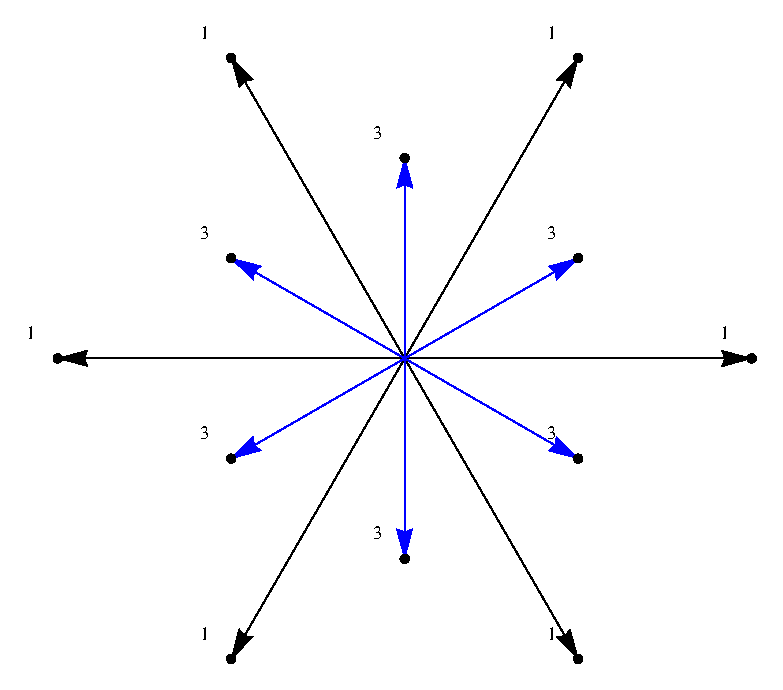
\includegraphics[width=80mm]{Special-A2-D4-all-2}
  }
  \caption{Projection of $D_{4}$ ($so(8)$)-root system onto root space of special subalgebra $A_{2}$
    ($su(3)$). Note that this roots system is $G_{2}$ but with non-trivial multiplicities. }
 \label{fig:d4-a2_splint}
\end{figure}


Relying on these theorems we can encode the projections of root system by Dynkin diagrams. We need
to allow simple roots to have non-trivial multiplicities. 

Classification of special embeddings

\begin{theorem}\label{va1}
Вложения
\begin{itemize}
\item $so(n-1)\rightarrow so(n)$,
\item $so(n)\rightarrow su(n)$,
\item $su(n)\rightarrow sp(2n)$,
\item $su(n-1)\rightarrow su(n)$,
\item $sp(n)\rightarrow su(2n)$
\end{itemize} -- все максимальные специальные вложения класса $A$ простых алгебр в простые алгебры (некоторые вкладываемые алгебры просты с точностью до фактора $u(1)$);
вложения
\begin{itemize}
\item $so(n)\oplus so(m)\rightarrow so(n+m)$
\item $su(n)\oplus su(m)\rightarrow su(n+m)$
\item $sp(n)\oplus sp(m)\rightarrow sp(n+m)$
\item $so(n)\oplus so(m)\rightarrow so(nm)$
\item $su(n)\oplus su(m)\rightarrow su(nm)$
\item $so(n)\oplus sp(m)\rightarrow sp(nm)$
\item $sp(n)\oplus sp(m)\rightarrow so(4nm)$
\end{itemize} -- все максимальные специальные вложения класса $A$ полупростых алгебр в простые алгебры \cite {sp1}.
\end{theorem}


\begin{theorem}\label{va2}
Не существует максимальных вложений класса $B$ полупростых (но не простых) алгебр в простые классические алгебры Ли. Если же вложение класса $B$ в простую алгебру $g$ строится на представлении $d$ размерности $p$, то оно может быть максимальным, только если $d$ неприводимо и:
\begin{itemize}
\item $g=so(n)$, $d$ -  ортогональное представление, $n=p$,
\item $g=sp(n)$, $d$ -  симплектичное представление, $n=p/2$,
\item $g=su(n)$, $d$ -  не ортогональное и не симплектичное представление, $n=p$.
\cite {sp1}
\end{itemize}
\end{theorem}

Эта теорема позволяет в подавляющем большинстве случаев определять максимальность вложения, не строя его явно.\\

Максимальные вложения класса $B$ приведены в таблице \ref{max-embeddings-class-B} (ну или еще какая-то текстовая связка-объяснение таблицы).


\begin{table}[h]

\label{max-embeddings-class-B}
\caption{Максимальные вложения класса $B$ в алгебры $so(2n)$, $so(2n-1)$, $su(n)$, $sp(2n)$ для $n\le 20$ \cite {sp1}.}
\begin{tabular}[t]{|p{3em}|p{20em}|}
\hline
 $a$ & $g$\\
\hline
$ sp(2)$ & $so(10)$, $so(14)$, $sp(8)$, $sp(10)$, $sp(20)$, $so(20)$  \\
\hline
$ su(3)$ & $su(6)$, $so(8)$, $su(10)$, $su(15)$, $so(27)$  \\
\hline
$ su(4)$ & $so(15)$, $su(10)$, $su(20)$, $so(20)$  \\
\hline
$ sp(3)$ & $so(14)$, $sp(7)$, $su(21)$ \\
\hline
$ so(7)$ & $so(8)$, $so(21)$, $so(27)$ \\
\hline
$ su(5)$ & $su(10)$, $su(15)$, $so(24)$ \\
\hline
$ sp(4)$ & $so(27)$, $so(36)$ \\
\hline
$ so(8)$ & $so(28)$, $so(35)$ \\
\hline
$ so(9)$ & $so(36)$ \\
\hline
$ su(6)$ & $su(15)$, $sp(10)$, $so(35)$ \\
\hline
$ so(10)$ & $su(16)$ \\
\hline
$ so(12)$ & $sp(16)$ \\
\hline
$ G_2$ & $so(7)$, $so(14)$ \\
\hline
$ F_4$ & $so(26)$ \\
\hline
\end{tabular}

\end{table}

\section{Splints for special embeddings}
\label{sec:splints-spec-embedd}



\begin{table}[h]
\begin{tabular}[t]{|p{2em}|p{6em}|p{5em}|p{5em}|p{2em}|p{6em}|}
\hline
Тип & $s$ & $W_a\subset W_s$ & $W_s\subset W_a$ & $g_{inv} $ & Примеры \\
\hline
1 & корневая система & нет & да & есть  & $B_2\rightarrow D_3$, $G_2\rightarrow B_3$\\
\hline
2 & корневая система  & да & да & нет & $A_1\rightarrow A_1+A_1$ \\
\hline
3 & корневая система  & да & нет & есть & $A_1+A_1\rightarrow D_3$ \\
\hline
4 & не корневая система  & да & нет & есть & $A_1\rightarrow A_2$, $A_1\rightarrow B_3$\\
\hline
5 & не корневая система  & да & нет & нет  & $A_1\rightarrow B_2$\\
\hline
6 & \multicolumn{4}{|l|}{$W_a\not\subset W_s$ и $W_s\not\subset W_a$} & $B_2\rightarrow D_4$\\
\hline
\end{tabular}
\caption{Классы специальных сплинтов.}
\label {spsp}
\end{table}


\section*{Conclusion}
\label{sec:conclusion}


\bibliography{special-bibliography}{} 
\bibliographystyle{apalike}
%%  \bibitem{d1}
%%  {\it Е.Б.Дынкин}
%%  Полупростые подалгебры полупростых алгебр.
%%  // Тр. Моск. матем. об-ва, т.1, стр. 39-166 (1952)
%%  \bibitem{d2}
%%  {\it Е.Б.Дынкин}
%%  Максимальные подгруппы классических групп.
%%  // Труды Моск. матем. об-ва, т. 1 (1952)
%%  
%%  
\end{document}
